
\section{\LARGE Постановка задачи}
Решение краевой задачи протекания газа через область $\Omega$

Система уравнений, описывающая нестационарное движение баротропного газа в области $\Omega$ размерности 2 или 3, выглядит следующим образом

\begin{figure}[h]
\center{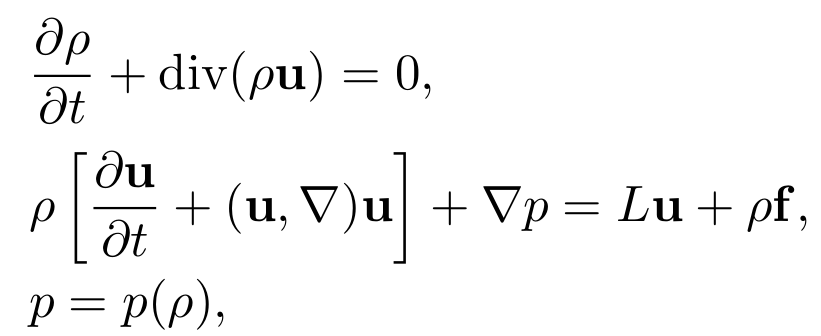
\includegraphics[width=0.4\linewidth]{./images/1.png}}
\end{figure}
где $L$ есть линейный симметричный положительно определенный оператор
\begin{figure}[h!]
\center{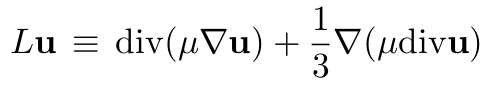
\includegraphics[width=0.35\linewidth]{./images/11.png}}
\end{figure}

Для построения разностной схемы в двумерном случае с односторонними разностями, направленными против потока, и вычисляемой функцией $g = ln(p)$ запишем систему в виде
\begin{figure}[h!]
\center{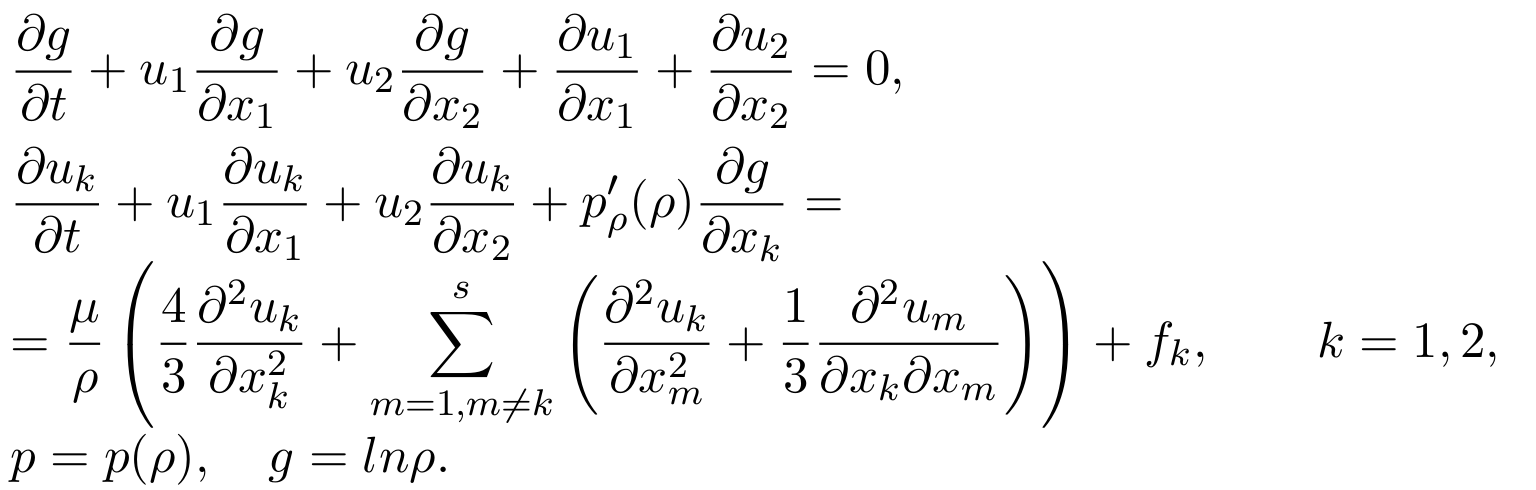
\includegraphics[width=0.8\linewidth]{./images/4.png}}
\end{figure}
\newpage
Неизвестные функции: плотность $p$ и вектор скорости $u$ являются функциями переменных Эйлера
\begin{figure}[h!] 
\center{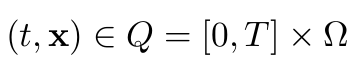
\includegraphics[width=0.27\linewidth]{./images/14.png}}
\end{figure}

В начальный момент времени задаются функции, значения которых определяют плотность и скорость газав каждой точке области $\Omega$:
\begin{figure}[h]
\center{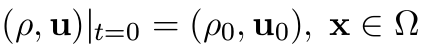
\includegraphics[width=0.3\linewidth]{./images/15.png}}
\end{figure}

\section{Область и граничные условия}
Компоненты функции скорости на границе области $\Omega$ будем считать равными нулю, если явно не задано другое условие. На границе, где вектор скорости направлен во внутрь, будем считать известной фукнцию плотности, положив её значение равным $\rho_{\gamma}$. На остальных участках границы функция плотности считается неизвестной и подлежит определению.

Обозначим через $\Omega_{nm}$ квадрат, координаты точек которого удовлетворяют неравенствам $n < x < n + 1$ и $m < y < m + 1$. Множества точек, составляюзие стороны квадрата $\Omega_{nm}$ обозначим $\Gamma^{x-}_{nm}$, $\Gamma^{x+}_{nm}$, $\Gamma^{y-}_{nm}$ и $\Gamma^{y+}_{nm}$, где индекс x или y означает, какая из координат на стороне является постоянной, а + или - означает максимальное или минимальное значение, которое принимает эта координата. С учетом этих обозначений область и начальные условия можно записать в следующем виде:
\begin{equation*}
\bar{\Omega} = \bar{\Omega}_{01}\cup\bar{\Omega}_{02}\cup\bar{\Omega}_{11}\cup\bar{\Omega}_{12}\cup\bar{\Omega}_{10}\cup\bar{\Omega}_{20};
\end{equation*}
\begin{equation*}
u_1(x, y) = w, \quad where \quad (x, y)\in \Gamma^{x-}_{01}\cup\Gamma^{x+}_{02};
\end{equation*}
\begin{equation*}
\dfrac{\partial u_2 (x, y)}{\partial y} = 0, \quad where \quad (x, y)\in \Gamma^{x+}_{20}
\end{equation*}



\section{\LARGE Алгоритм}

Используемые обозначения:
\begin{figure}[h!]
\center{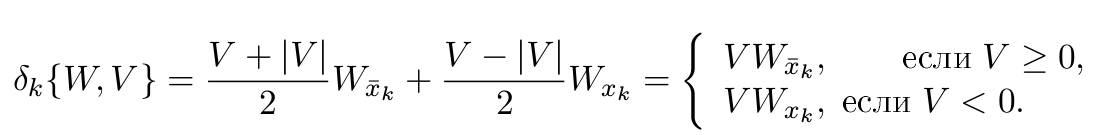
\includegraphics[width=0.6\linewidth]{./images/17.png}}
\center{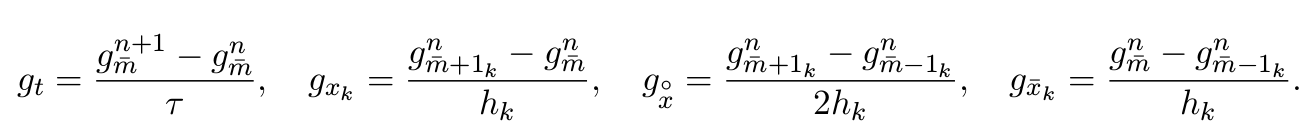
\includegraphics[width=0.8\linewidth]{./images/18.png}}
\end{figure} \\
Для поиска численного решения задачи предлагается использовать р.с.:
\begin{figure}[h!]
\center{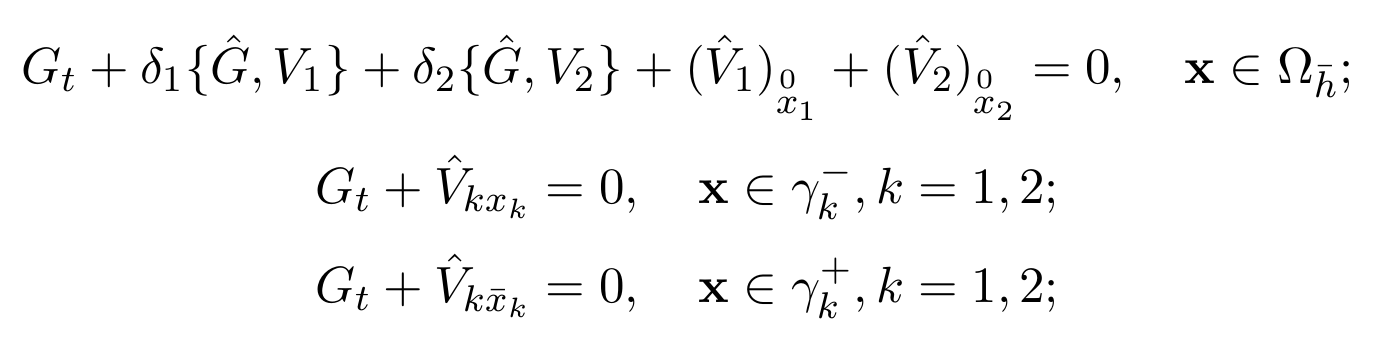
\includegraphics[width=0.6\linewidth]{./images/7.png}}
\center{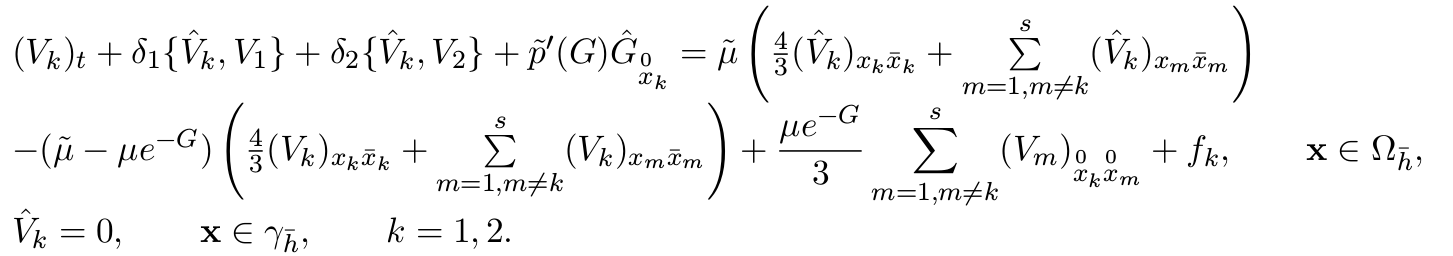
\includegraphics[width=0.9\linewidth]{./images/8.png}}
\end{figure} 
\begin{figure}[h!]
\center{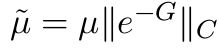
\includegraphics[width=0.16\linewidth]{./images/9.png}}
\end{figure} \\
\newpage
Приведем индексную запись уравнений данной разностной схемы:
\begin{figure}[h!]
\center{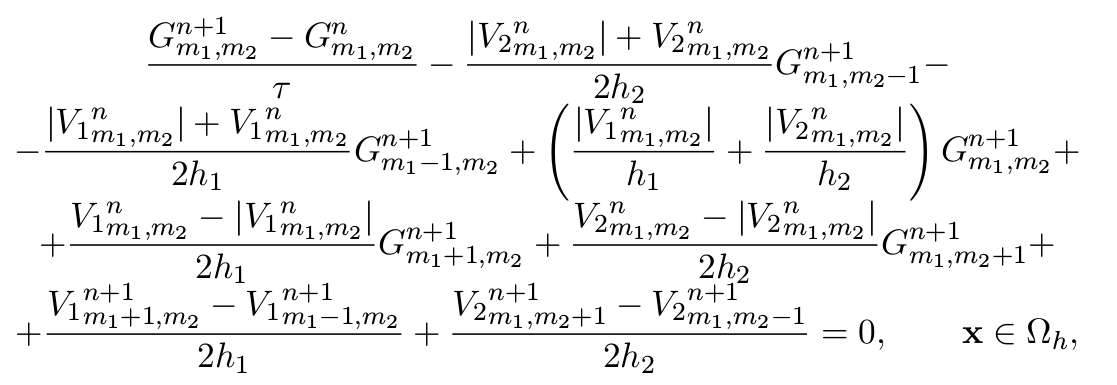
\includegraphics[width=0.75\linewidth]{./images/2.png}}
\end{figure}
\begin{figure}[h!]
\center{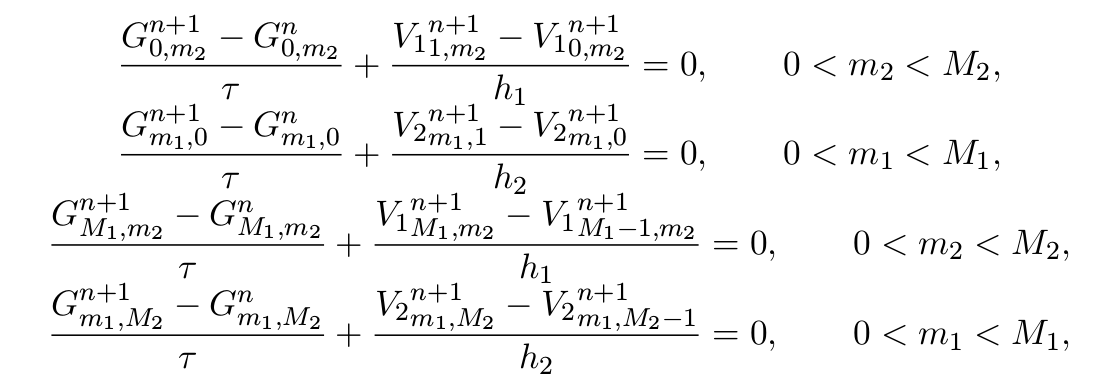
\includegraphics[width=0.75\linewidth]{./images/3.png}}
\end{figure}
\begin{figure}[h!]
\center{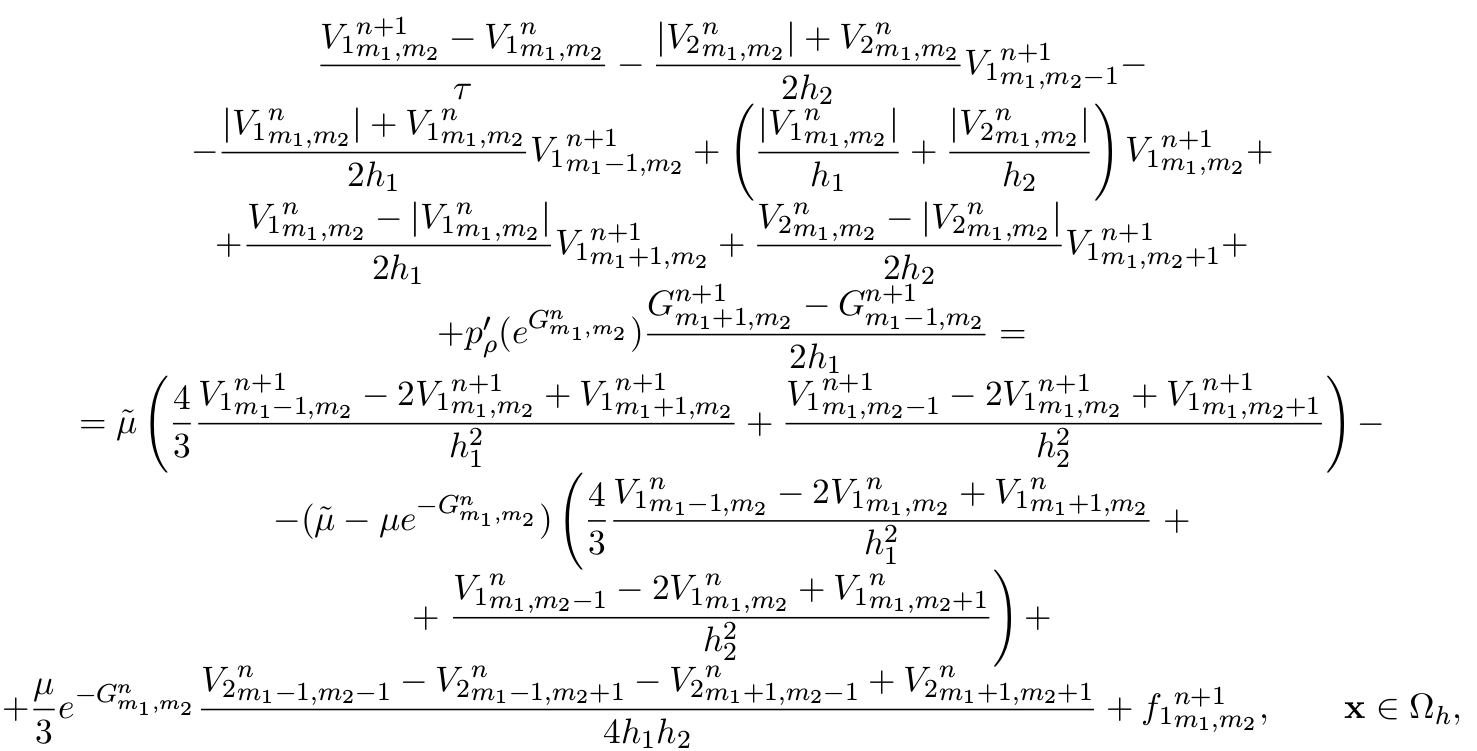
\includegraphics[width=0.95\linewidth]{./images/19.png}}
\end{figure}
\newpage
\begin{figure}[h!]
\center{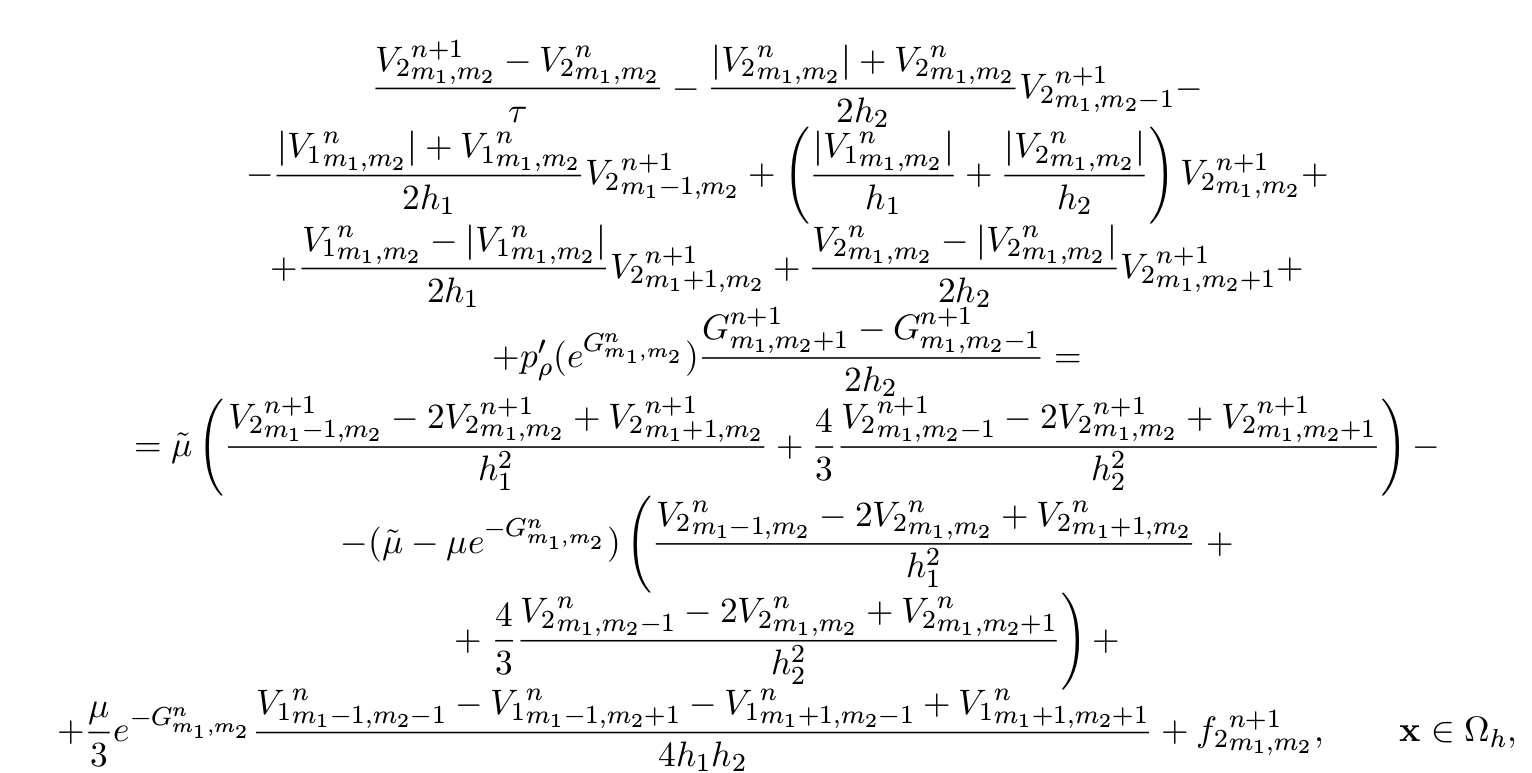
\includegraphics[width=0.95\linewidth]{./images/5.png}}
\end{figure} 
Данные уравнения образуют СЛАУ, решая которую находим сеточное решение на очередном слое.

Из первого разностного уравнения получаем следующие алгебраические уравнения для всех внутренних узлов:
\begin{figure}[h!]
{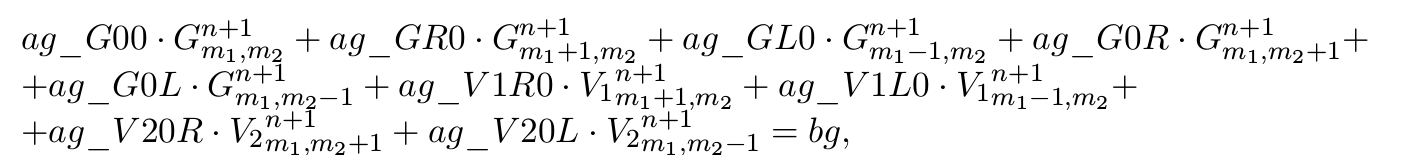
\includegraphics[width=0.93\linewidth]{./images/6.png}}
\end{figure} \\
где коэффициенты определяются по формулам:
\begin{figure}[h!]
{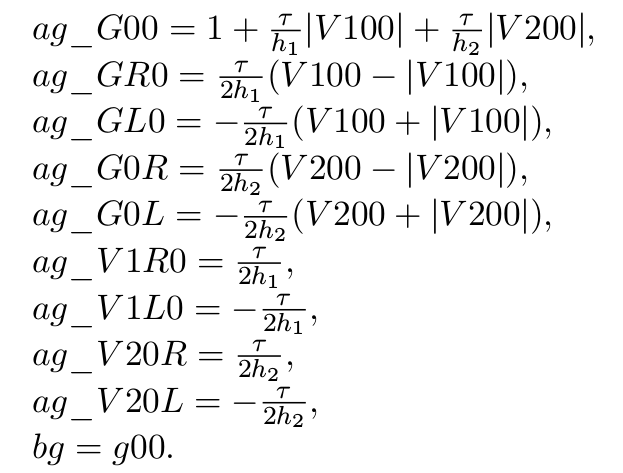
\includegraphics[width=0.38\linewidth]{./images/20.png}}
\end{figure} \\
Из третьего уравнения получаем: \\ \\
$ av1\_V100 \cdot (V_1)_{m_1,m_2}^{n+1} + av1\_V1R0 \cdot (V_1)_{m_1+1,m_2}^{n+1}
+ av1\_V1L0 \cdot (V_1)_{m_1-1,m_2}^{n+1} + av1\_V10R \cdot (V_1)_{m_1,m_2+1}^{n+1}
+ av1\_V10L \cdot (V_1)_{m_1,m_2-1}^{n+1} + av1\_GR0 \cdot G_{m_1 + 1,m_2}^{n+1}
+ av1\_GL0 * G_{m_1-1,m_2}^{n+1} = bv1,$ \\ \\
где \\ \\
$ av1\_V100 = 1 + \frac{\tau}{h_1}|V100| + \frac{\tau}{h_2}|V200| +  \tilde{\mu}\tau(\frac{8}{3h_1^2} + \frac{2}{h_2^2}) $ \\
$ av1\_V1L0 = -\frac{\tau}{2h_1}(|V100| + V100) - \frac{4\tilde \mu\tau}{3h_1^2} $ \\
$ av1\_V10L = -\frac{\tau}{2h_2}(|V200| + V200) - \frac{\tilde \mu\tau}  {h_2^2}  $ \\
$ av1\_V1R0 =  \frac{\tau}{2h_1}(V100 - |V100|) - \frac{4\tilde \mu\tau}{3h_1^2} $ \\
$ av1\_V10R =  \frac{\tau}{2h_2}(V200 - |V200|) - \frac{\tilde \mu\tau}  {h_2^2}  $ \\
$ av1\_GR0  =  \frac{\tau}{2h_1}\rho_p' $ \\
$ av1\_GL0  = -\frac{\tau}{2h_1}\rho_p' $
\begin{multline*}
bv1 = V100 + (-\tilde \mu + \mu e^{-g})(\frac{4\tau}{3h_1^2}(V1L0 - 2V1 + \\ +
  V1R0) + \frac{\tau}{h_2^2}(V10L - 2V1 + V10R)) +
  \\ + \frac{\mu\tau e^{-g}}{12h_1h_2}(V2LL - V2LR - V2RL + V2RR) + \tau F_{v2}
\end{multline*}
Из четвертого уравнения получаем: \\ \\
$ av2\_V200 \cdot (V_2)_{m_1,m_2}^{n+1} + av2\_V2R0 \cdot (V_2)_{m_1+1,m_2}^{n+1}
+ av2\_V2L0 \cdot (V_2)_{m_1-1,m_2}^{n+1} + av2\_V20R \cdot (V_2)_{m_1,m_2+1}^{n+1}
+ av2\_V20L \cdot (V_2)_{m_1,m_2-1}^{n+1} + av2\_GR0 \cdot G_{m_1 + 1,m_2}^{n+1}
+ av2\_GL0 * G_{m_1-1,m_2}^{n+1} = bv1,$ \\ \\
где \\ \\
$ av2\_V200 = 1 + \frac{\tau}{h_1}|V100| + \frac{\tau}{h_2}|V200| +  \tilde{\mu}\tau(\frac{8}{3h_2^2} + \frac{2}{h_1^2})$ \\
$ av2\_V2L0 = -\frac{\tau}{2h_1}(|V100| + V100) - \frac{\tilde \mu\tau}  {h_1^2}  $ \\
$ av2\_V20L = -\frac{\tau}{2h_2}(|V200| + V200) - \frac{4\tilde \mu\tau}{3h_2^2} $ \\
$ av2\_V2R0 =  \frac{\tau}{2h_1}(V100 - |V100|) - \frac{\tilde \mu\tau}  {h_1^2}  $ \\ 
$ av2\_V20R =  \frac{\tau}{2h_2}(V200 - |V200|) - \frac{4\tilde \mu\tau}{3h_2^2} $ \\
$ av2\_G0R  =  \frac{\tau}{2h_2}\rho_p'e^g $ \\
$ av2\_G0L  = -\frac{\tau}{2h_2}\rho_p'e^g $
\begin{multline*}
bv2 = V200 - (\tilde \mu - \mu e^{-g})(\frac{\tau}{h_1^2}(V2L0 - 2V2 +
\\ + V2R0) + \frac{4\tau}{3h_2^2}(V20L - 2V2 + V20R)) +
\\ + \frac{\mu\tau e^{-g}}{12h_1h_2}(V1LL - V1LR - V1RL + V1RR) + \tau F_{v2}
\end{multline*}